\documentclass{standalone}
\usepackage{tikz}
\usepackage{amssymb}
\usetikzlibrary{decorations.markings}

\begin{document}

\centering

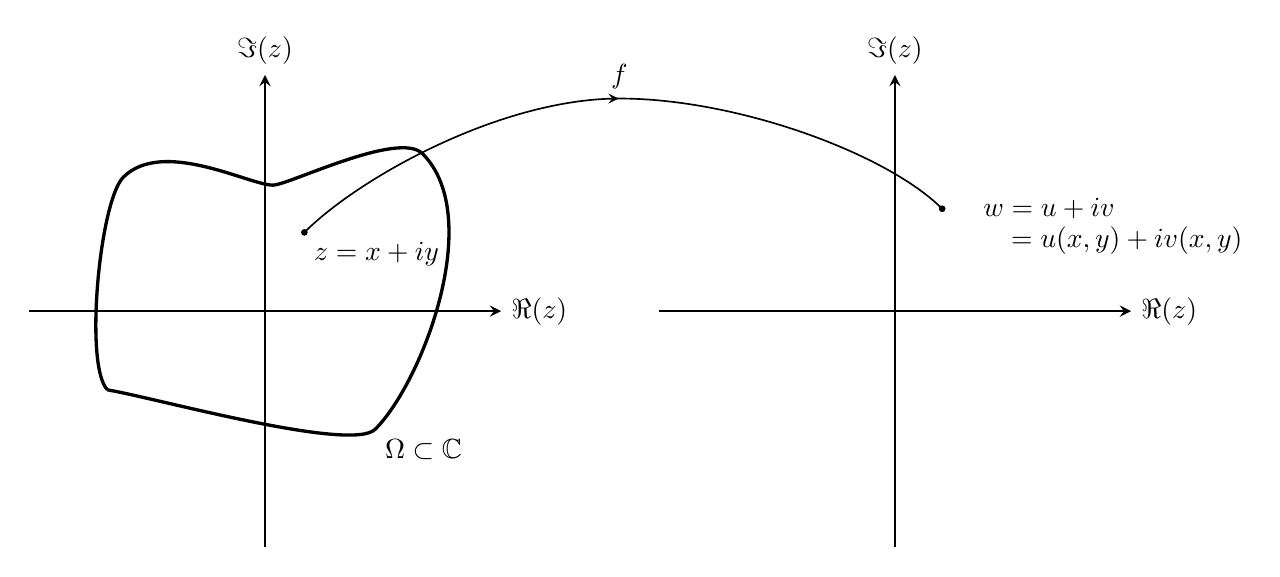
\begin{tikzpicture}
    \tikzset{
    every node/.style={font=\normalsize, text=black},
    arrowstyle/.style={->, >=stealth}}
    % Axes
    \draw [thick, arrowstyle](-4,-3) -- (-4,3) node[above]{$\Im(z)$};
    \draw [thick, arrowstyle](-7,0) -- (-1,0) node[right]{$\Re(z)$};
    \draw [thick, arrowstyle](4,-3) -- (4,3) node[above]{$\Im(z)$};
    \draw [thick, arrowstyle](1,0) -- (7,0) node[right]{$\Re(z)$};
    % Omega area
    \draw[black, very thick] (-6,-1) 
        .. controls (-6.3,-0.7) and (-6.1,1.4) .. (-5.8,1.7) 
        .. controls (-5.3,2.2) and (-4.2,1.6) .. (-3.9,1.6)
        .. controls (-3.7,1.6) and (-2.3,2.3) .. (-2,2)
        .. controls (-1.2,1.2) and (-2.0,-0.9) .. (-2.6,-1.5)
        .. controls (-2.9,-1.8) and (-5.4,-1.1) .. (-6,-1);
    \node[below right,black] at (-2.6,-1.5) {$\Omega \subset \mathbb{C}$};
    \coordinate (z) at (-3.5, 1);    
    \draw[fill=black] (z) circle (1pt);
    \node[below right] at (z) {$z=x+iy$};
    \coordinate (w) at (4.6, 1.3);
    \coordinate (p) at (4.6, 0.9); %nieuw node introduceren onder de andere voor 2de deel tekstblok
    \draw[fill=black] (w) circle (1pt);
    \node[right, xshift=0.4cm] at (w) {$w=u+iv$};
    \node[right, xshift=0.4cm] at (p) {$\quad =u(x,y)+iv(x,y)$};%quad zorgt dat gelijk aan tekens onder elkaar komen
    % transformation arrow
    \draw[postaction={decorate}, decoration={markings,mark=at position 0.5 with {\arrow{stealth}}}]
    [black, semithick] (z)
    .. controls (-2.8,1.7) and (-1,2.7) .. (0.5,2.7)
    .. controls (2,2.7) and (3.9,2) .. (w);
    \node[above,black] at (0.5,2.7) {$f$};
\end{tikzpicture}
\end{document}  